\label{chapt:prelim}

In this foregoing section, methods used to set up the analytical approach are discussed in detail. Please note that all parameters used in this section will follow Table~\ref{table:prelim_params}.

%----------------------------------------------------------------------------------------------------------------------
\section{Deflection \& Differential Relations}

The first key equation to setting up the differential relations is taken from \cite{nisbett2014shigley}. Equation~\ref{eq:Mcurve} shows the relationship between internal bending moment on a beam and its radius of curvature. 

\begin{equation}
	\label{eq:Mcurve}
	\frac{1}{\rho}=\frac{M}{EI}
\end{equation}

Where $1/\rho$ is the radius of curvature defined as Equation~\ref{eq:curve} \cite{nisbett2014shigley}. Note that for a small differential, the denominator approaches unity, leaving the final result.

\begin{equation}
	\label{eq:curve}
	\frac{1}{\rho}=\frac{d^2y/dx^2}{\left( 1 +(dy/dx)^2 \right)^\frac{3}{2}} \approx \frac{d^2y}{dx^2}
\end{equation}

From Equation~\ref{eq:curve} deflection $y(x)$ relations for slope \ref{eq:slope}, moment \ref{eq:mmt} and shearing force \ref{eq:shr} as a consequence \cite{nisbett2014shigley}.

\begin{equation}
	\label{eq:slope}
	\theta(x) = \frac{dy}{dx}
\end{equation}

\begin{equation}
	\label{eq:mmt}
	M(x) = EI\ \frac{d\theta(x)}{dx} = EI\ \frac{d^2y}{dx^2}
\end{equation}

\begin{equation}
	\label{eq:shr}
	V(x) = \frac{dM(x)}{dx} = EI\ \frac{d^3y}{dx^3}
\end{equation}

The above listed equations are important for understand how deflection translates to other internal loading.\\

Furthermore, boundary conditions (BC) may be derived as a result. The following equations assume that the boundary in question is located at $x_0$.\\

\textbf{Free Ends:} no loading, allowed to deform\\
\begin{equation}
	\label{eq:2_freeBC}
	\begin{aligned}
		y(x_0) = y_0          \\
		\theta(x_0)= \theta_0 \\
		M(x_0) = 0            \\
		V(x_0) = 0            
	\end{aligned}
\end{equation}

\textbf{Simply Supported:} free to rotate\\
\begin{equation}
	\label{eq:2_endBC}
	\begin{aligned}
		y(x_0)= 0            \\
		\theta(x_0)=\theta_0 \\
		M(x_0)= 0            \\
		V(x_0) =V_0          
	\end{aligned}
\end{equation}

\textbf{Fixed:} load is carried at the ends\\
\begin{equation}
	\label{eq:2_fixedBC}
	\begin{aligned}
		y(x_0)=0      \\
		\theta(x_0)=0 \\
		M(x_0)=M_0    \\
		V(x_0) =V_0   
	\end{aligned}
\end{equation}

The equations from this subsection serve as an important set up for the more complex approach derived in the following section. 

%----------------------------------------------------------------------------------------------------------------------
\section{Theory of Cylindrical Shells}
\label{section:3_shells}

As per \cite{timoshenko1959theory}, this section covers the method of approximating the drum barrel as a long thin cylindrical shell. With this assumption, the governing ordinary differential equation (ODE) is derived. First, the following coordinate system is presented as per Figure~\ref{fig:CoordSyst} below. Note that all symbols and steps in this subsquent derivation will follow \cite{timoshenko1959theory}.

\begin{figure}[H]
	\centering
	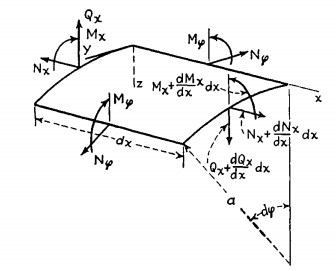
\includegraphics[width=0.6\textwidth]{CoordSyst}
	\caption[Coordinate system adopted for derivation of ODE.]{Coordinate system adopted for derivation of ODE.\protect\cite{timoshenko1959theory}}
	\label{fig:CoordSyst}
\end{figure}

From the above figure, the differential area of the cylindrical shell is presented as Equation~\ref{eq:diffsurf}. Note that in the foregoing section, $x$ is the axial direction, $a$ is the shell's outer radius and $\varphi$ is the circumferential direction.
 
\begin{equation}
	\label{eq:diffsurf}
	dA = dS\ dx = a\ d\varphi \ dx   
\end{equation}

Equilibrium is performed as a force balance in the $x, z$ axes and moment balance about the $y$ axis and presented as Equations ~\ref{eq:eqbrm_x}, ~\ref{eq:eqbrm_z}, ~\ref{eq:eqbrm_y} respectively. Note that $Z$ denotes and external pressure applied to the shell (not shown in Figure~\ref{fig:CoordSyst}).

\begin{equation}
	\label{eq:eqbrm_x}
	\frac{dN_x}{dx}\ a\ d\varphi \ dx = 0
\end{equation}

\begin{equation}
	\label{eq:eqbrm_z}
	\frac{dQ_x}{dx}\ a\ d\varphi \ dx+ N_\varphi \ a\ d\varphi \ dx +Z\ a\ d\varphi \ dx= 0
\end{equation}

\begin{equation}
	\label{eq:eqbrm_y}
	\frac{dM_x}{dx}\ a\ d\varphi \ dx- Q_x\ a\ d\varphi \ dx= 0
\end{equation}

First looking at \ref{eq:eqbrm_x}, the axial force $N_x$ is determined by taking the integral with respect to $x$ \ref{eq:eqbrm_x2}. 

\begin{equation}
	\label{eq:eqbrm_x2}
	N_x = C = 0 
\end{equation}

The above equation states that the effects of bending due to the axial forces are neglected, which is a valid assumption for thin shells \cite{timoshenko1959theory}.\\

Similarly with \ref{eq:eqbrm_z} and \ref{eq:eqbrm_y}, simplifications will lead to \ref{eq:eqbrm_z2} and \ref{eq:eqbrm_y2} respectively.
\begin{equation}
	\label{eq:eqbrm_z2}
	\frac{dQ_x}{dx}+\frac{1}{a}\ N_\varphi = -Z
\end{equation}

\begin{equation}
	\label{eq:eqbrm_y2}
	\frac{dM_x}{dx}- Q_x= 0
\end{equation} 

Next, differential relations between displacement and strain are presented in Equation~\ref{eq:strain_xphi}. Note $u$ and $w$ are displacements in both $x$ and $z$ directions.

\begin{equation}
	\label{eq:strain_xphi}
	\begin{aligned}
		\varepsilon_x = \frac{du}{dx}      \\
		\varepsilon_\varphi = -\frac{w}{a} 
	\end{aligned}
\end{equation}

From Hooke's law $N_x$ may be also written as Equation~\ref{eq:Hookes_Nx}. Substituting Equation~\ref{eq:strain_xphi} will yield the following. Note that $h$ represents the thickness of the cylindrical shell.
\begin{equation}
	\label{eq:Hookes_Nx}
	N_x = \frac{Eh}{1-\nu^2}\ \left( \varepsilon_x + \nu \varepsilon_\varphi \right) =  \frac{Eh}{1-\nu^2}\ \left( \frac{du}{dx} -\nu \ \frac{w}{a} \right)
\end{equation} 

%%%%%%%%%%%%%%%%%%%%%%%%%%%%%%%%%%%%%%%%%%%%%%%%%
Solving Equation~\ref{eq:Hookes_Nx} using ~\ref{eq:eqbrm_x2} leaves \ref{eq:Nx_simpl}.
\begin{equation}
	\label{eq:Nx_simpl}
	\frac{du}{dx} =  \nu \ \frac{w}{a}
\end{equation} 

Similarly, with $N_\varphi$, again applying \ref{eq:strain_xphi} leaves \ref{eq:Nphi_simpl}.
\begin{equation}
	\label{eq:Hookes_Nphi}
	N_\varphi = \frac{Eh}{1-\nu^2}\ \left( \varepsilon_\varphi + \nu \varepsilon_x \right) = \frac{Eh}{1-\nu^2}\  \left( -\frac{w}{a}+\nu \ \frac{du}{dx} \right)
\end{equation} 

\begin{equation}
	\label{eq:Nphi_simpl}
	N_\varphi = - \frac{Ehw}{a}
\end{equation}

As a result of no change in curvature in the $\varphi$ direction, we know that $\frac{dM_\varphi}{d\varphi}= 0$ hence no change in the circumferential moments \cite{timoshenko1959theory}. This relation is translated to axial moments $M_x$ with \ref{eq:Mphix}.

\begin{equation}
	\label{eq:Mphix}
	\begin{aligned}
		M_\varphi = \nu M_x        \\
		M_x = -D \frac{d^2w}{dx^2} 
	\end{aligned}
\end{equation}

Where $D$ is defined as the flexural rigidity of the shell \ref{eq:flexrig}. This term replaces the $EI$ term from Equations~\ref{eq:Mcurve} - \ref{eq:shr}.

\begin{equation}
	\label{eq:flexrig}
	D \triangleq \frac{Eh^3}{12(1-\nu^3)}
\end{equation}

Simplifying \ref{eq:eqbrm_z2} to get $Q_x = \frac{dM_x}{dx}$, the following is put in \ref{eq:eqbrm_y2} to get the final ODE in Equation~\ref{eq:de1}

\begin{equation}
	\label{eq:de1}
	\begin{aligned}
		\frac{d^2M_x}{dx^2}+\frac{1}{a} \ N_\varphi = -Z \\
		D\ \frac{d^4w}{dx^4}+\frac{Eh}{a^2} \ w = Z      \\
		\frac{d^4w}{dx^4}+\beta^4 \ w = \frac{Z}{D}      
	\end{aligned}
\end{equation} 

Where $\beta^4$ is some parameter defined as \ref{eq:betaquad}.

\begin{equation}
	\label{eq:betaquad}
	\beta^4 \triangleq \frac{Eh}{4a^2D}= \frac{3(1-\nu^2)}{a^2h^2}
\end{equation}

The solution to this common fourth order, linear, non-homogeneous, ODE in \ref{eq:de1} has a general solution of Equation~\ref{eq:solnDE} \cite{timoshenko1959theory}.

\begin{equation}
	\label{eq:solnDE}
	w(x)=e^{\beta x} \left(C_1 \cos \beta x +C_2 \sin \beta x \right)+e^{-\beta x} \left(C_3 \cos \beta x +C_4 \sin \beta x \right) +f(x)
\end{equation}

Where $ C_1, C_2, C_3, C_4$ are integration constants to be solved based on BC and $f(x)$ is the particular solution to the ODE (recall $y_{general}=y_{homogeneous}+y_{particular}$).\\

In the following section, a specific solution of this differential equation will be determined.

%----------------------------------------------------------------------------------------------------------------------

\section{Roark's Solution}
\label{section:3_roark}

The previous equation prepared the set up to the solution procedure outlined in Example 3 of Chapter 12, p.538 \cite{roarks}. A similar solution was developped in an Excel \cite{EXCEL} calculator (see Appendix B).The main important factor lies in the assumptions of a long shell(i.e. $\beta l \geq 6$) and a TWPV (i.e $R/t \geq 10$).\\

Referring to Appendix B, a final calculated value of $t=1.686 \Unit{in}= 42.8 \Unit{mm}$ upon confirming the assumptions.

\section{Roark's Buckling}
\label{section:3_buckle}

Up to this point, all values for calculating the drum barrel thickness have focused on the stress state. It was proposed by John Umina to investigate buckling. To confirm that stress is primary mode of failure, a linear buckling analysis is completed.\\

With equations from Table 35 of \cite{roarks}, the following relations are presented. First, Equation~\ref{eq:3_buckle1} is presented for a long thin tube under uniform external pressure with ends simply supported.
\begin{equation}
	\label{eq:3_buckle1}
	p' =\frac{1}{4} \frac{E}{1-\nu^2} \frac{t^3}{R^3}
\end{equation}

To classify as a long tube, the length of the barrel $L$ must be greater the critical length as calculated with Equation~\ref{eq:3_lcrit}.
\begin{equation}
	\label{eq:3_lcrit}
	L' = 4.90 R \sqrt{\frac{R}{t}}
\end{equation}

For the studied range of $t \in [0.05, 1.05] \Rightarrow L < L' \therefore$ Equation~\ref{eq:3_buckle2} must is to calculate the critical buckling pressure for a short thin cylinder.

\begin{equation}
	\label{eq:3_buckle2}
	p' =0.807\  \frac{Et^2}{LR}\  \sqrt[4]{\left( \frac{1}{1-\nu^2} \right)^3 \left( \frac{t}{R}\right)^2}
\end{equation}

With \ref{eq:3_buckle2} and the aforementioned thickness range, critical pressure values were computed with the \cite{PYTHON} script in Appendix~\ref{appendix:a4}. These results are displayed in the following plot (see Figure~\ref{fig:3_buckling}).

\begin{figure}[H]
	\centering
	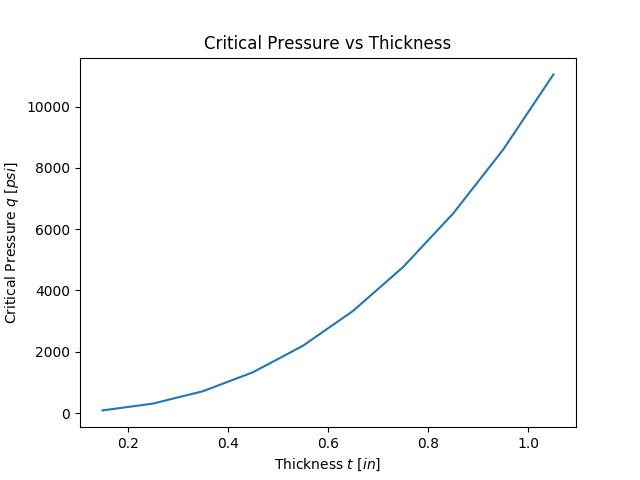
\includegraphics[scale=0.75]{3_buckling}
	\caption{Variation of critical buckling pressure $p'$ with $t$.}
	\label{fig:3_buckling}
\end{figure}

As depicted in the above figure, a very low thickness is required to achieve a critical buckling pressure $p'$ of $137\Unit{psi} \/\ 9.484\Unit{MPa}$ (as per Equation~\ref{eq:2_preq}).\\

By rearranging, \ref{eq:3_buckle2} for $t$ and setting $p'=1376\Unit{psi}$, a critical thickness of $0.418\Unit{in}= 10.6\Unit{mm}$ is required to avoid buckling. Based on these conclusions, buckling will not be the primary failure mode for the drum barrel given the loading scenario. The following section will validate all conclusions with a series of FEA simulations.



